\documentclass[tikz,border=10pt,12pt,x11names]{standalone}
\usepackage{tikz}
\usetikzlibrary{circuits.logic.US} % TiKZ Library for US Logic Circuits.
\begin{document}

	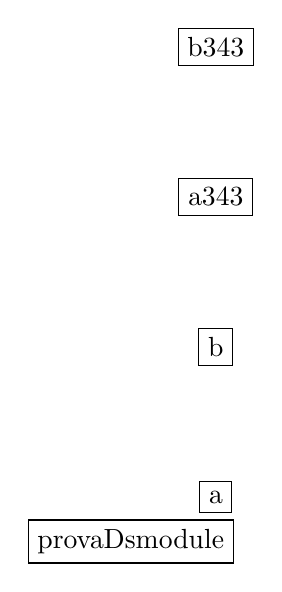
\begin{tikzpicture}[circuit logic US,
						tiny circuit symbols,
						every circuit symbol/.style={
						fill=white,draw}]

		\node[draw] at (-2.0bp,2.0bp) {provaDsmodule};

		\node[draw] (a) at (28.597bp,18.0bp) {a};
		\node[draw] (b) at (28.597bp,72.0bp) {b};
		\node[draw] (a343) at (28.597bp,126.0bp) {a343};
		\node[draw] (b343) at (28.597bp,180.0bp) {b343};


	\end{tikzpicture}

\end{document}